% Inbuilt themes in beamer
\documentclass{beamer}

% to make a box around formulas
\usepackage{empheq}

%Renumber backup slides
\usepackage{appendixnumberbeamer}

% Theme choice:
\usetheme{CambridgeUS}

% Title page details: 
\title{Präsentation Masterarbeit} 
\subtitle{Reanalysis of the 2019 $B^0 \longrightarrow  D^{*-}\ell^+ \nu_{\ell}$ data from Belle and extraction of the Cabibbo-Kobayashi-Maskawa matrix element $|V_{cb}|$}
\author{Hannes Kößl}
\institute[TU Wien]{Institut für Hochenergiephysik (HEPHY, Wien)}
\date{\today}
\logo{\large \LaTeX{}}


\begin{document}

% Title page frame
\begin{frame}
    \titlepage 
\end{frame}

% Remove logo from the next slides
\logo{}


% Outline frame
\begin{frame}{Inhalt}
    \tableofcontents
\end{frame}

\section{CKM Matrix}
\begin{frame}{CKM Matrix}
\begin{itemize}
    \item CKM Matrix

\begin{columns}
\column{.5\textwidth}
\Large
\begin{align*}
\textbf{V}=
\left(
\begin{array}{ccc}
 V_{\text{ud}} & V_{\text{us}} & V_{\text{ub}} \\
 V_{\text{cd}} & V_{\text{cs}} & V_{\text{cb}} \\
 V_{\text{td}} & V_{\text{ts}} & V_{\text{tb}} \\
\end{array}
\right)
\end{align*}
\normalsize
\column{0.5\textwidth}
\begin{figure}[htbp]
   \centering
    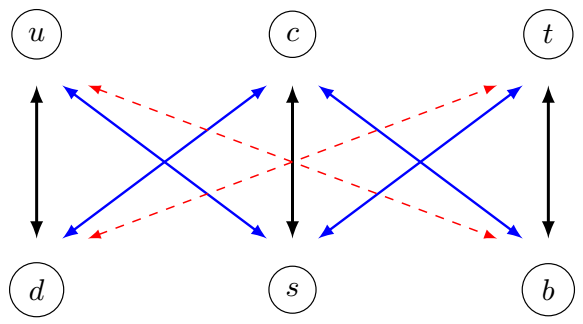
\includegraphics[width=0.65\textwidth]{./Bilder/CKM6}
   
    \label{fig:ink_exk}
\end{figure}  
\end{columns}
\vspace{0.5cm}
\item Bestimmung von $|V_{cb}|$
\begin{columns}
\column{.5\textwidth}
\centering \textbf{inklusiv}\\
$B\rightarrow X_c \ell \nu_{\ell}$
\column{.5\textwidth}
\centering \textbf{exklusiv}\\
$B\rightarrow D \ell \nu_{\ell}$\\
$B\rightarrow D^* \ell \nu_{\ell}$

\end{columns}
\end{itemize}
\end{frame}

%%%%%%%%%%%%%%%%%%%%%%%%%%%%%%%%%%%%%%%%%%%%%%%%%%%%%%%
\begin{frame}{CKM Matrix}
%\begin{figure}[htbp]
%   \centering
%    \includegraphics[width=0.5\textwidth]{./Bilder/vub_vcb_excl_2021}   
%    \label{fig:ink_exk}
%\end{figure}  
\begin{itemize}
    \item 3.3$\sigma$ Abweichung zwischen exklusiver und inklusiver Bestimmung von $|V_{cb}|$
\end{itemize}
\end{frame}

%%%%%%%%%%%%%%%%%%%%%%%%%%%%%%%%%%%%%%%%%%%%%%%%%%%%%%%
\section{Belle-Experiment}
\begin{frame}{Belle-Experiment}
\begin{columns}
\column{.5\textwidth}
%\begin{figure}[htbp]
%   \centering
%    \includegraphics[width=1.1\textwidth]{./Bilder/icondetector}
%\end{figure}  
\column{.45\textwidth}
  \begin{itemize}
    \item  { KEKB: asymmetrischer Elektronen-Positronen-  Beschleuniger}
  \item  {Laufzeit: 1999-2010}
    \item  {Schwerpunktsenergie: 10.58GeV ($\Upsilon(4S)$ Resonanz)}
  \item  {$\mathcal{L}_{peak}=2.1 \times 10^{34} cm^{-2} s^{-1}$}
  \item  {$\int \mathcal{L} dt > 1000 fb^{-1}  $}

  \end{itemize}
\end{columns}
\end{frame}

%%%%%%%%%%%%%%%%%%%%%%%%%%%%%%%%%%%%%%%%%%%%%%%%%%%%%%%
\begin{frame}{$B^0\longrightarrow D^{*-} \ell ^+ \nu_{\ell}$}
\begin{columns}
\column{.6\textwidth}
\begin{itemize}
\item
Messung von $|V_{cb}|$ mit Hilfe des exkusive semileptonische Zerfall $B^0 \longrightarrow D^{*-}\ell^+ \nu_{\ell}$ $(\ell = e, \mu)$
\item
Differenzielle Zerfallsrate ist eine Funktion vom handonischen Rückstoß w und den drei Winkel $\theta_{\ell}, \theta_{\nu}$ und $\chi$\\
\begin{align*}
\frac{d \Gamma   (B^0\longrightarrow D^{*-} \ell ^+ \nu_{\ell})}{dw d \cos \theta_l d \cos \theta_{\nu}d \chi}= f(w, \theta_{\ell}, \theta_{\nu}, \chi)
\end{align*}
\begin{align*}
w=\frac{P_B \cdot P_{D^*}}{m_B m_{D^*}}=\frac{m_B^2+m_{D^*}^2-q^2}{2 m_B m_{D^*}},
\label{eq:recoil}
\end{align*}
\end{itemize}
\column{.4\textwidth}
%\begin{figure}[htbp]
%   \centering
%    \includegraphics[width=0.7\textwidth]{./Bilder/feyn_dslnu}
%\end{figure} 
%\begin{figure}[htbp]
%   \centering
%    \includegraphics[width=0.7\textwidth]{./Bilder/angles_new}
%\end{figure} 
%$\theta_l$: Winkel zwischen $\ell$ und W Boson\\
%$\theta_{\nu}$: Winkel zwischen $D^0$ und $D^*$
\end{columns}
\end{frame}


%%%%%%%%%%%%%%%%%%%%%%%%%%%%%%%%%%%%%%%%%%%%%%%%%%%%%%%
\section{Formfaktor-Parametrisierung}
\begin{frame}{Formfaktor-Parametrisierung}
\begin{itemize}
\item Caprini, Lellouch, Neubert (CLN) Parametrisierung\\
\item Parameter: $\rho^2$, $R_1(1)$, $R_2(1)$, $F(1)|Vcb|\eta_{EW}$
%\fbox{\parbox{1cm}{
\item Formfatoren und Formfaktor-Verhältnise
\small
\begin{empheq}[box=\fbox]{align*}
        h_{\text{A1}} (w) & = h_{\text{A1}} (1) \left[1 - 8 \rho^2 z + (53 \rho^2 - 15) z^2 - (231 \rho^2 - 91) z^3  \right] \\
		R_1(w) & = R_1(1) - 0.12(w-1)+0.05(w-1)^2 \\
		R_2(w) & = R_2(1) + 0.11(w-1)-0.06(w-1)^2
\end{empheq}
%}}
\item Belle 2019 Publikation:
\small
\center
\begin{tabular}{cc}
\hline
Parameter & Messung  \\
\hline

$\rho ^2$    	&	$1.106 \pm 0.031 \pm 0.007$	\\

$R_1(1)$		&	$1.229 \pm 0.028 \pm 0.009$	 \\
$R_2(1)$		&	$0.852 \pm 0.021 \pm 0.006$	 \\
$\mathcal{F} (1) |V_{cb}| \eta _{\text{EW}} \times 10^3$		&	$35.06 \pm 0.15 \pm 0.56.$	\\ 
\hline
\end{tabular} 

\end{itemize}
\end{frame}

%%%%%%%%%%%%%%%%%%%%%%%%%%%%%%%%%%%%%%%%%%%%%%%%%%%%%%%
\section{Fit}
\begin{frame}{Fit}
\begin{itemize}
\item
Vierdimensionaler Fit in den Variablen w, $\cos(\theta_l)$, $\cos(\theta_{\nu})$ und $\chi$
\begin{align*}
\chi^2=\sum_{i,j}(N_i^{obs}-N_i^{exp})C_{ij}^{-1}(N_j^{obs}-N_j^{exp})
\end{align*}
\item Bin-Einteilung
\small
\begin{center}
\begin{tabular}[h]{r@{}c@{}lcr@{}c@{}lc}
\hline
\multicolumn{3}{c}{\textit{bin index}}
& \multicolumn{1}{c}{\textit{variable}}
& \multicolumn{3}{c}{\textit{range}}
& \multicolumn{1}{c}{\textit{width}}\\
\hline
  1&...&10 & w &  $1.00\,$ &...& $\,1.50$ & 0.05 \\  
    11&...&20 & $\cos(\theta_l)$ & $-1.0\,$ &...& $\,+1.0$ & 0.2\\    
    21&...&30 & $\cos(\theta_{\nu})$ & $-1.0\,$ &...& $\,+1.0$ & 0.2\\    
    31&...&40 & $\chi$ & $-\pi\,$ &...& $\,+\pi$ & $2 \pi/10$\\   
\hline
\end{tabular}\\
\end{center}
\normalsize
\vspace{0.2cm}
\item Vier verschiedene Konfigurationen:

40 bin Fit, 37 Bin Fit, nur statischtische Fehler, d'Agostini bias
\end{itemize}


\end{frame}


%%%%%%%%%%%%%%%%%%%%%%%%%%%%%%%%%%%%%%%%%%%%%%%%%%%%%%%
\section{Ergebnisse}
\begin{frame}{Ergebnisse}
\begin{columns}
\column{.5\textwidth}
\begin{figure}[htbp]
   \centering
    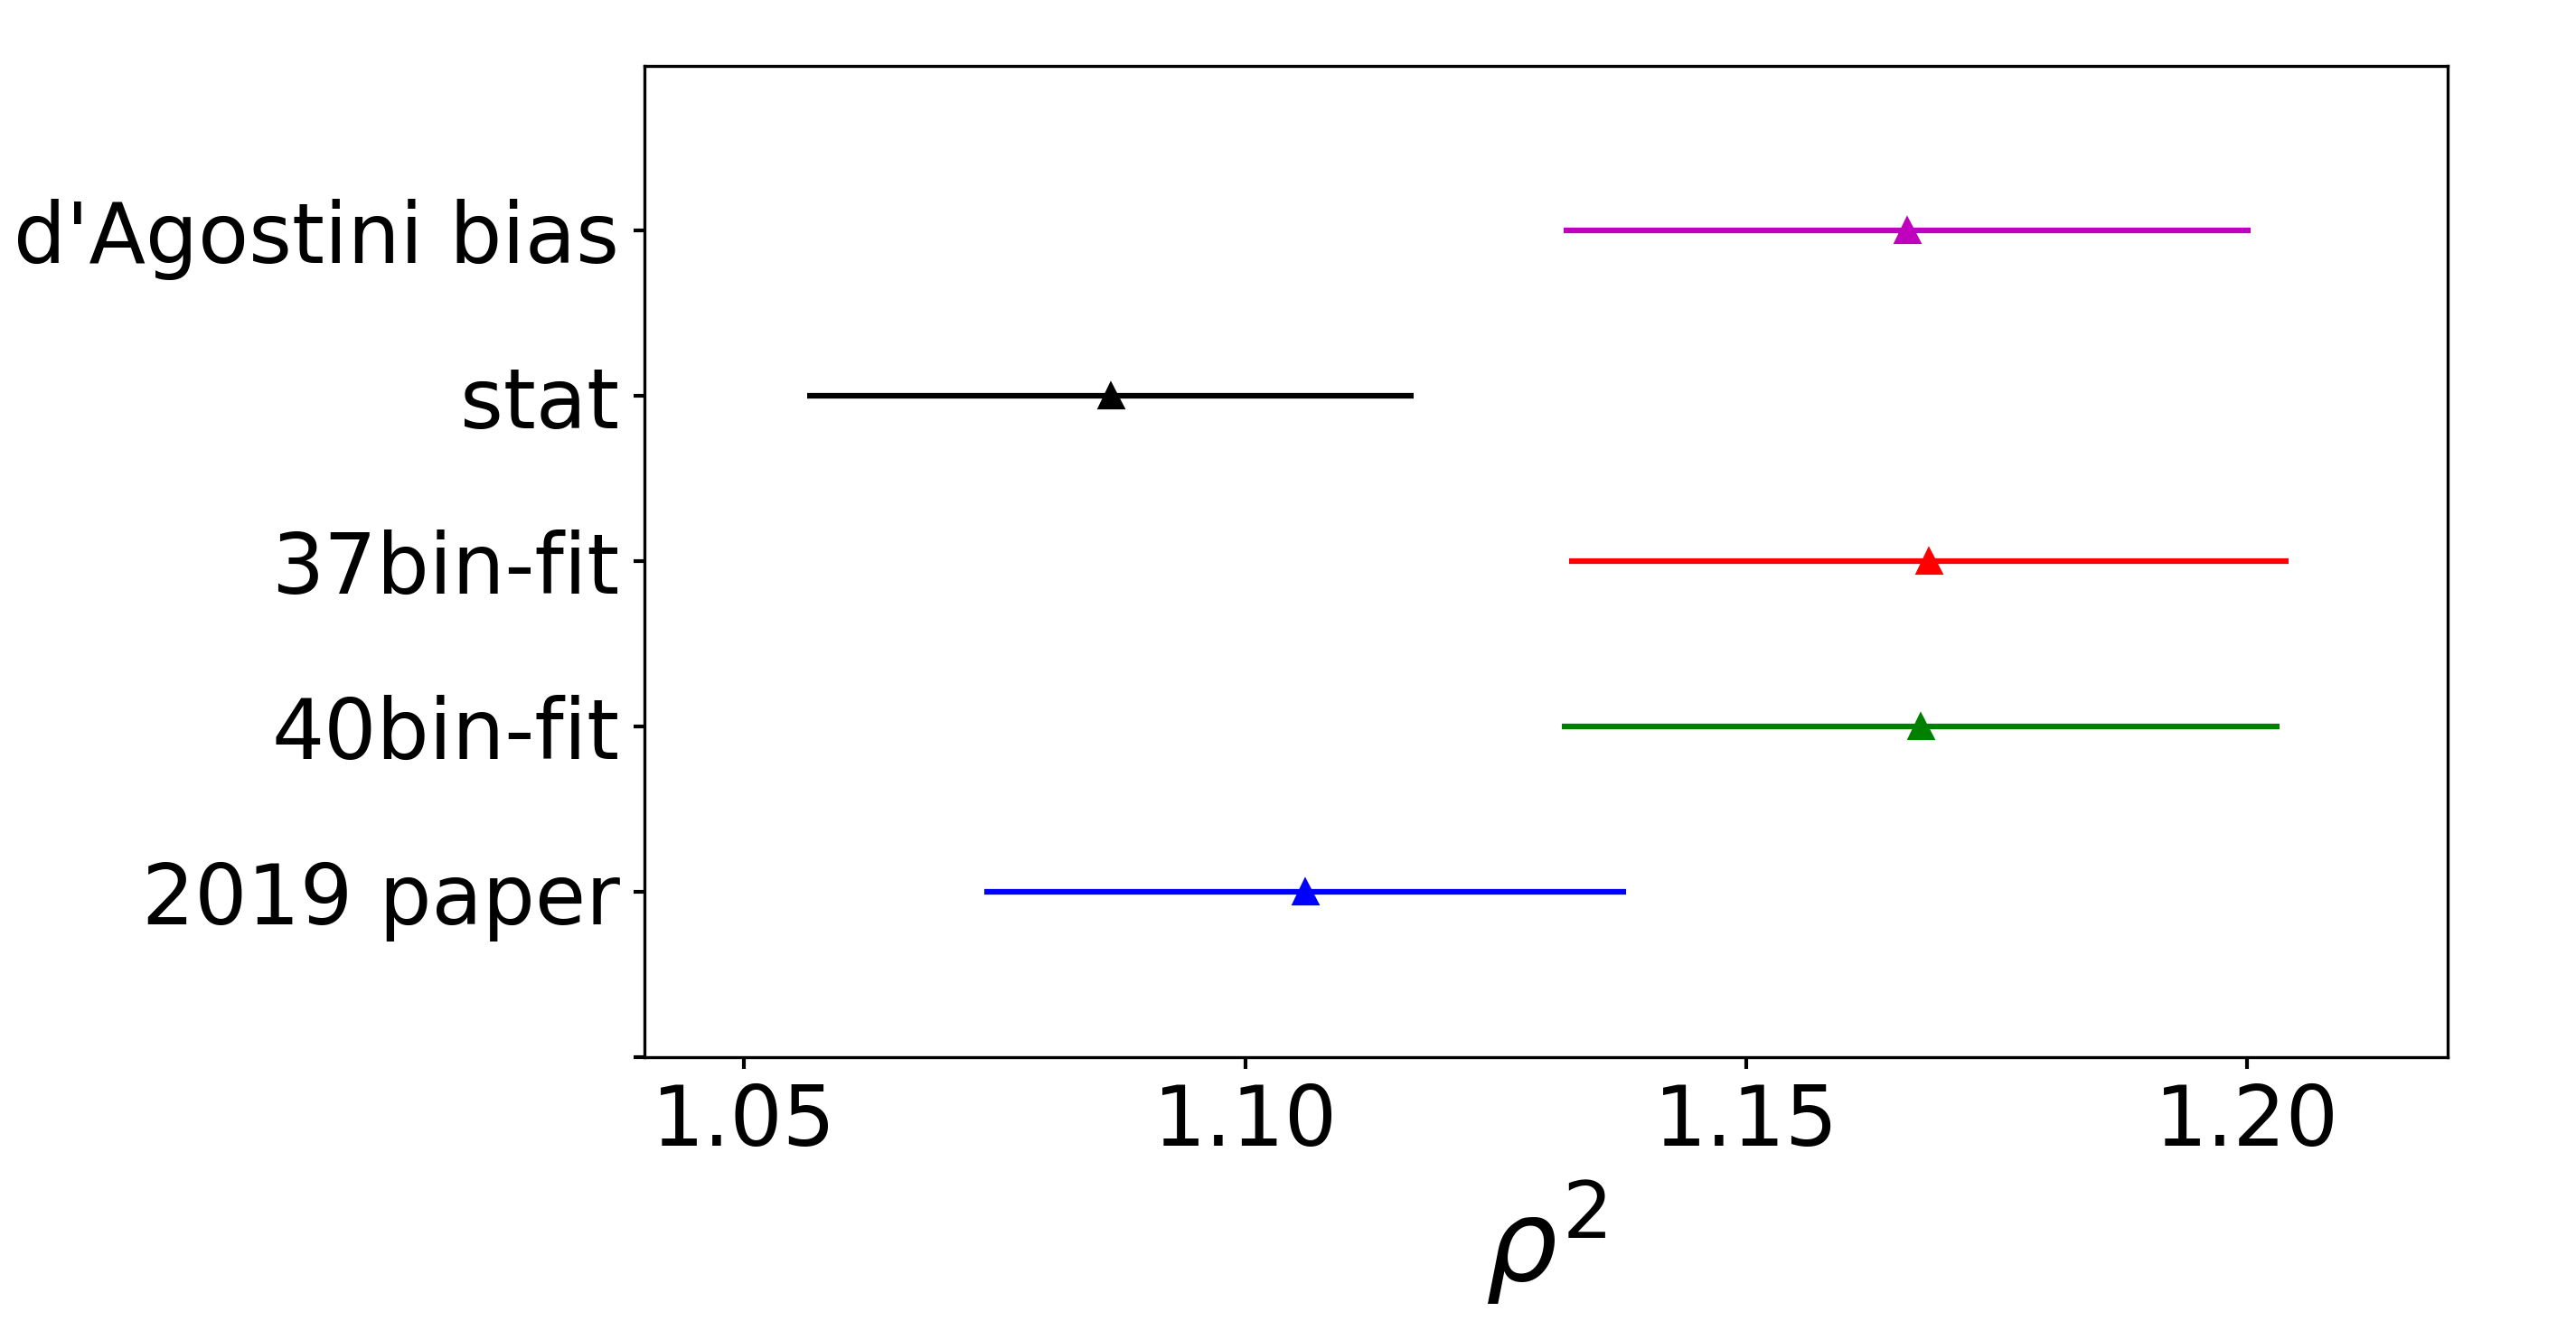
\includegraphics[width=1.0\textwidth]{./Bilder/CLN_all_1}
    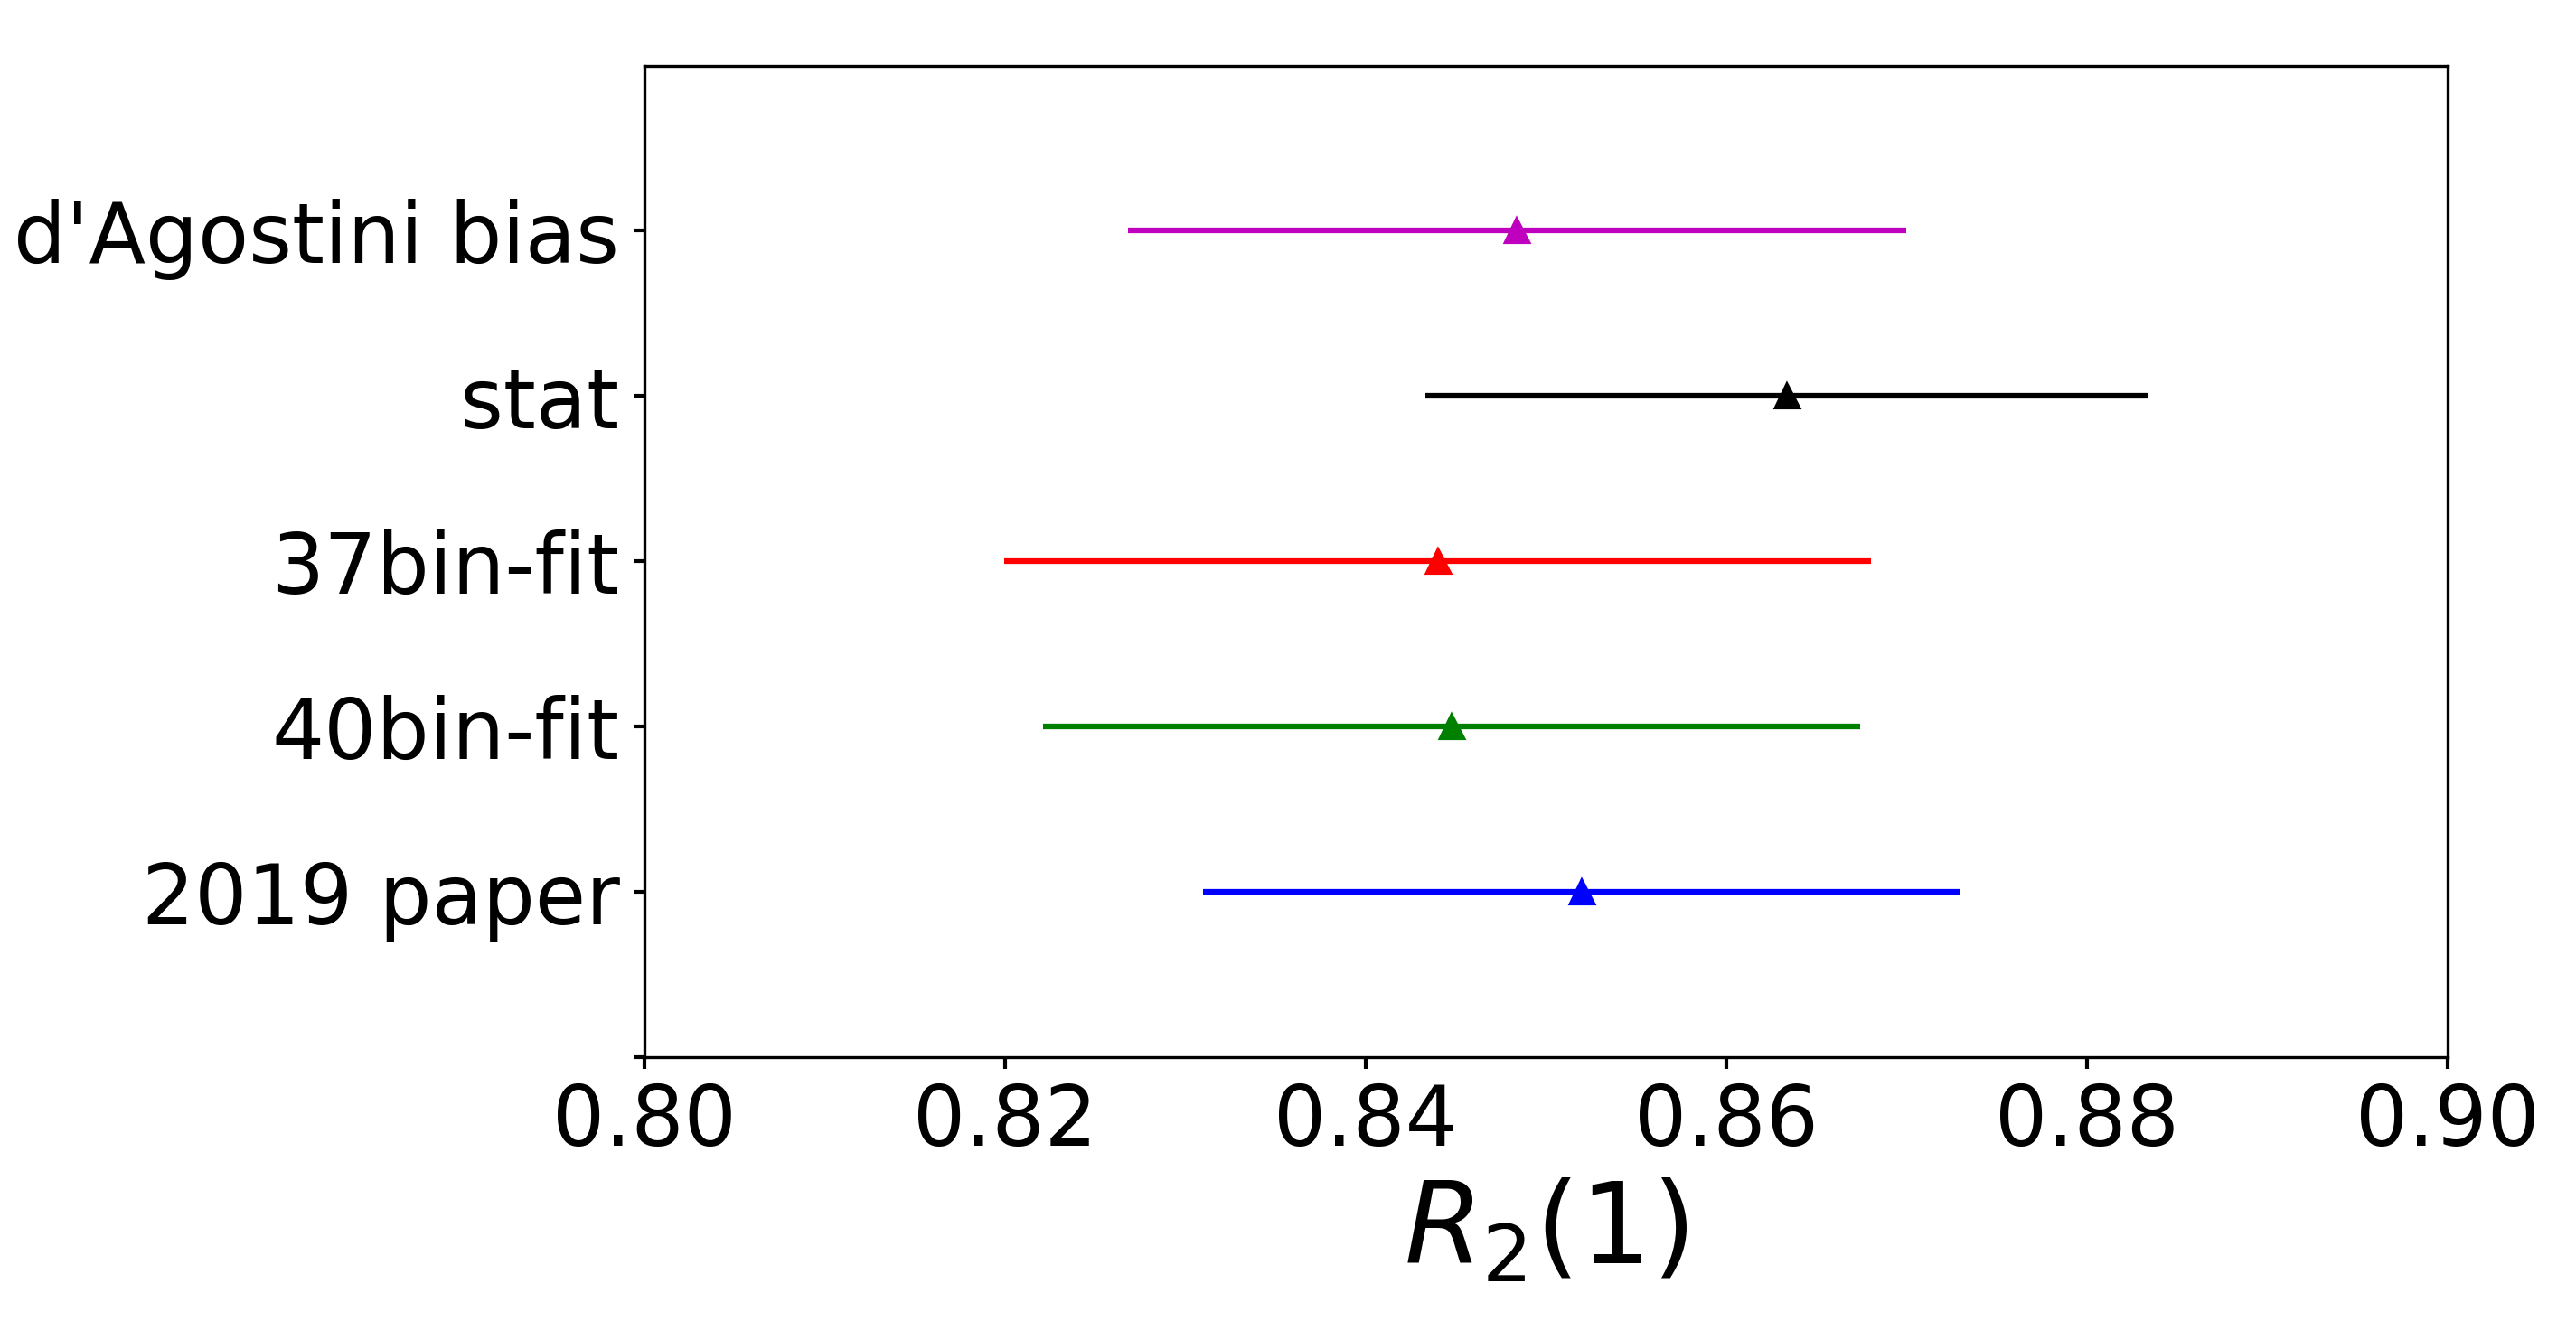
\includegraphics[width=1.0\textwidth]{./Bilder/CLN_all_3}
\end{figure}  
\column{.5\textwidth}
\begin{figure}[htbp]
   \centering
    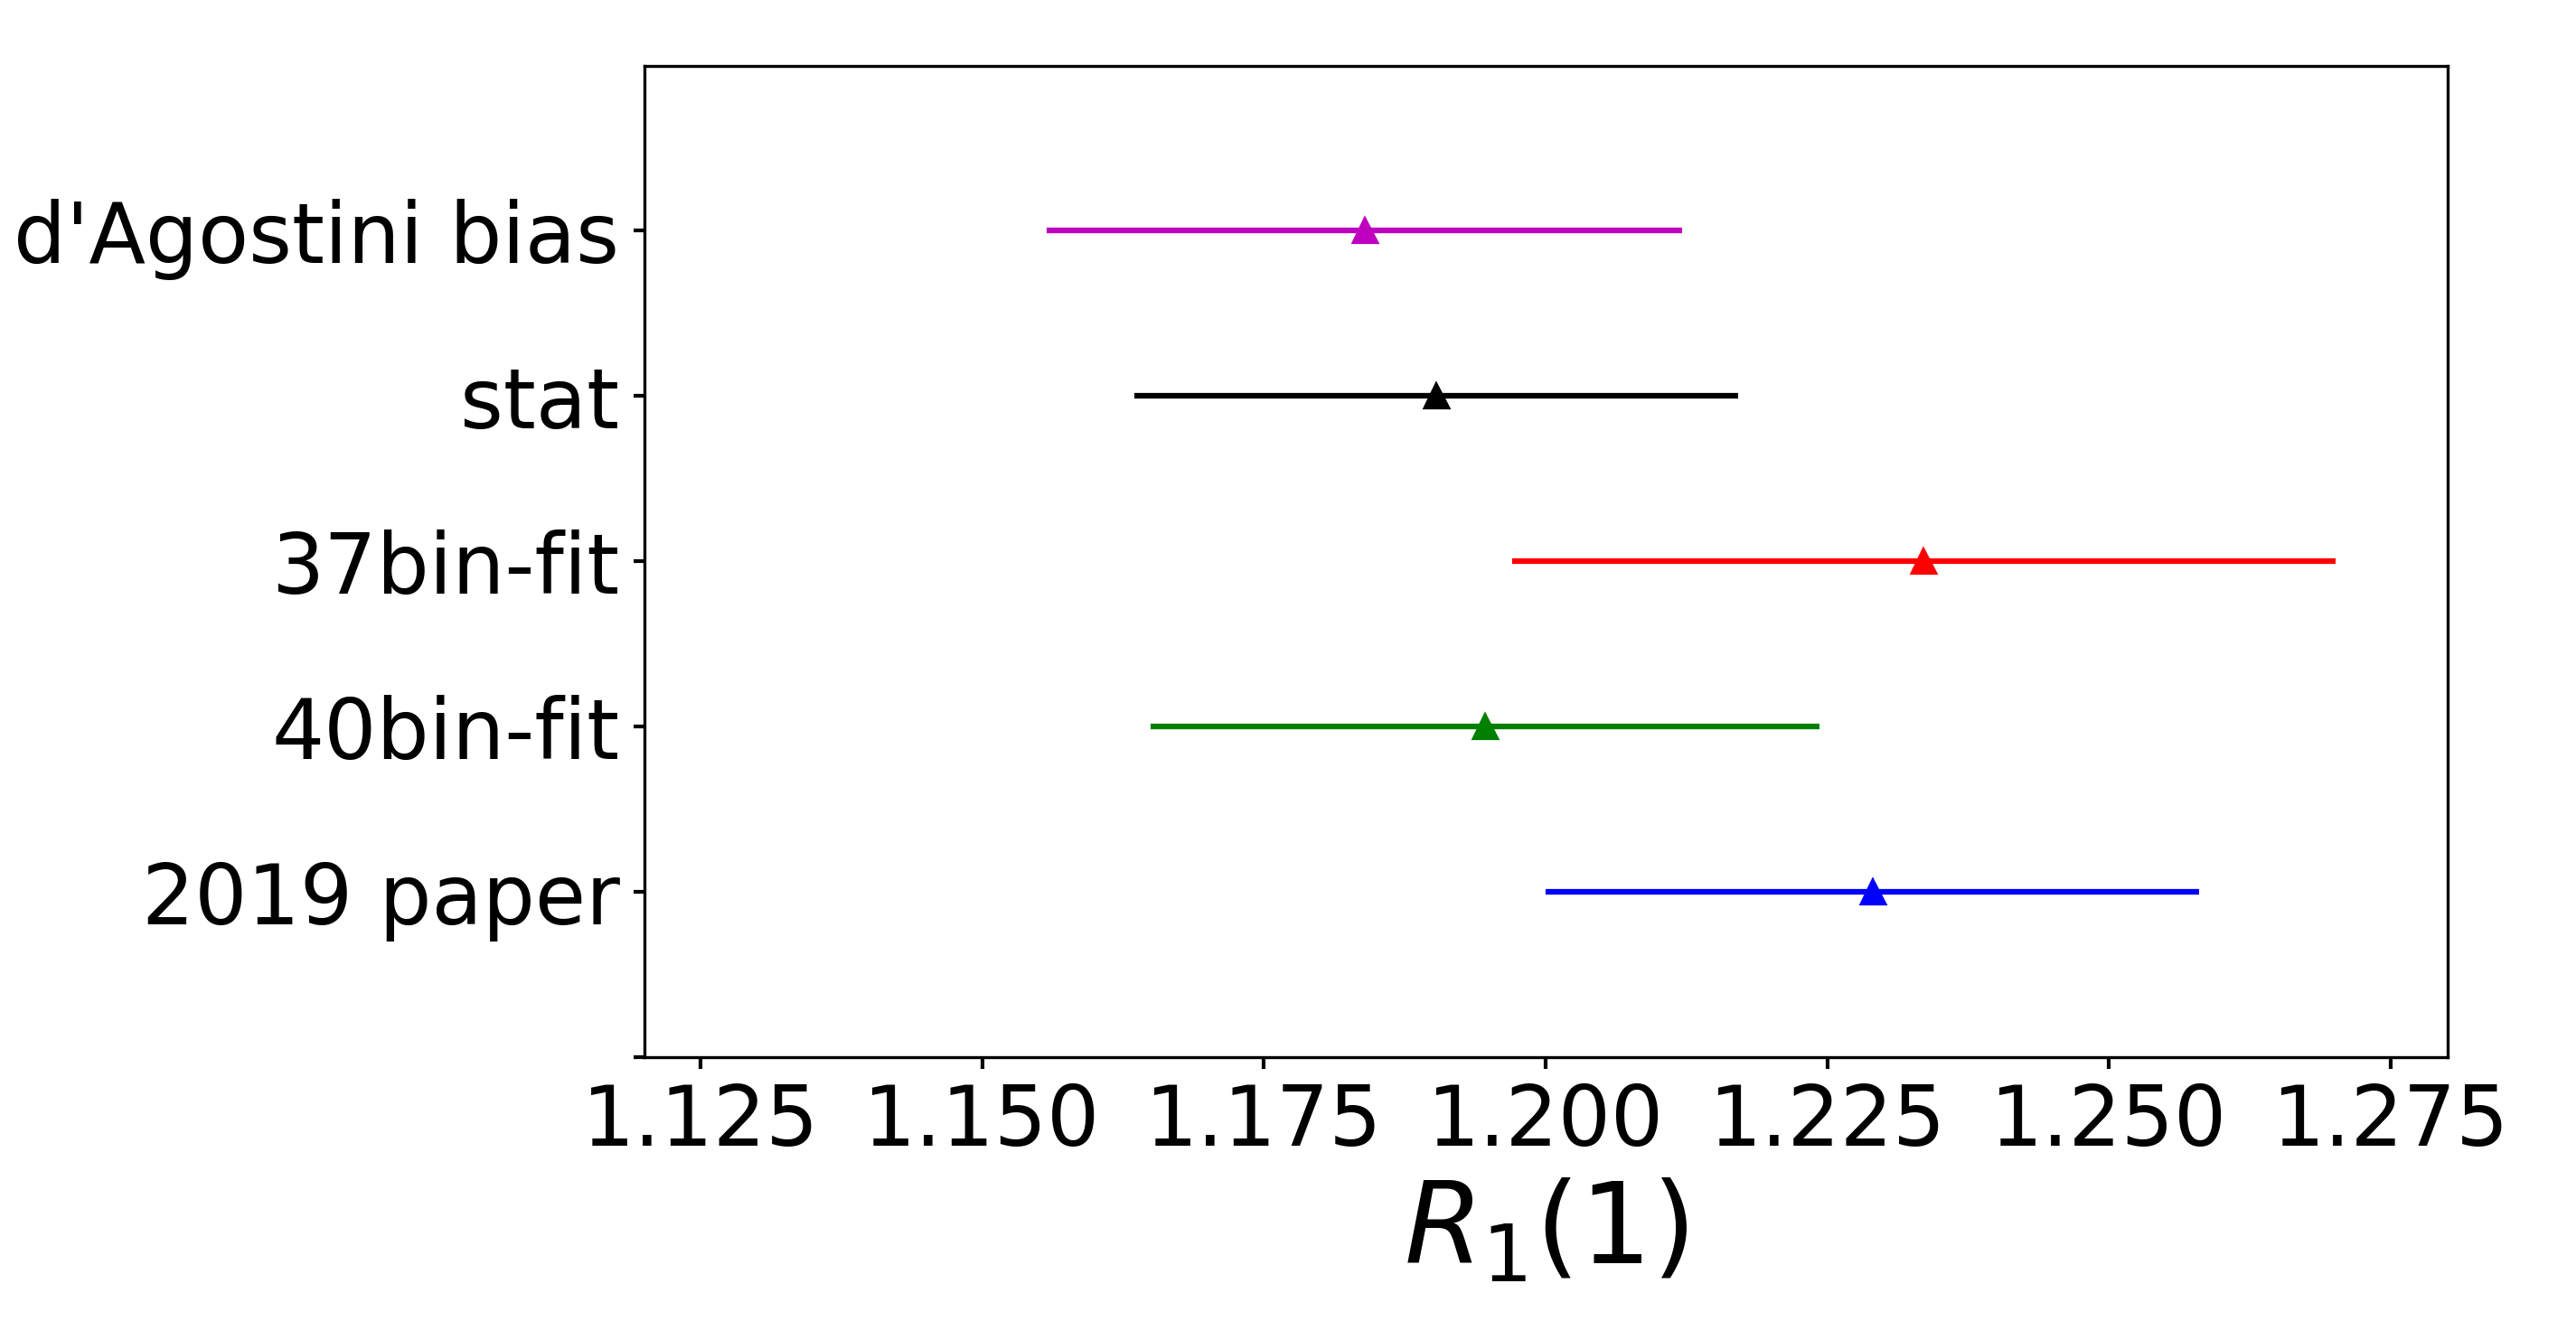
\includegraphics[width=1.0\textwidth]{./Bilder/CLN_all_2}
    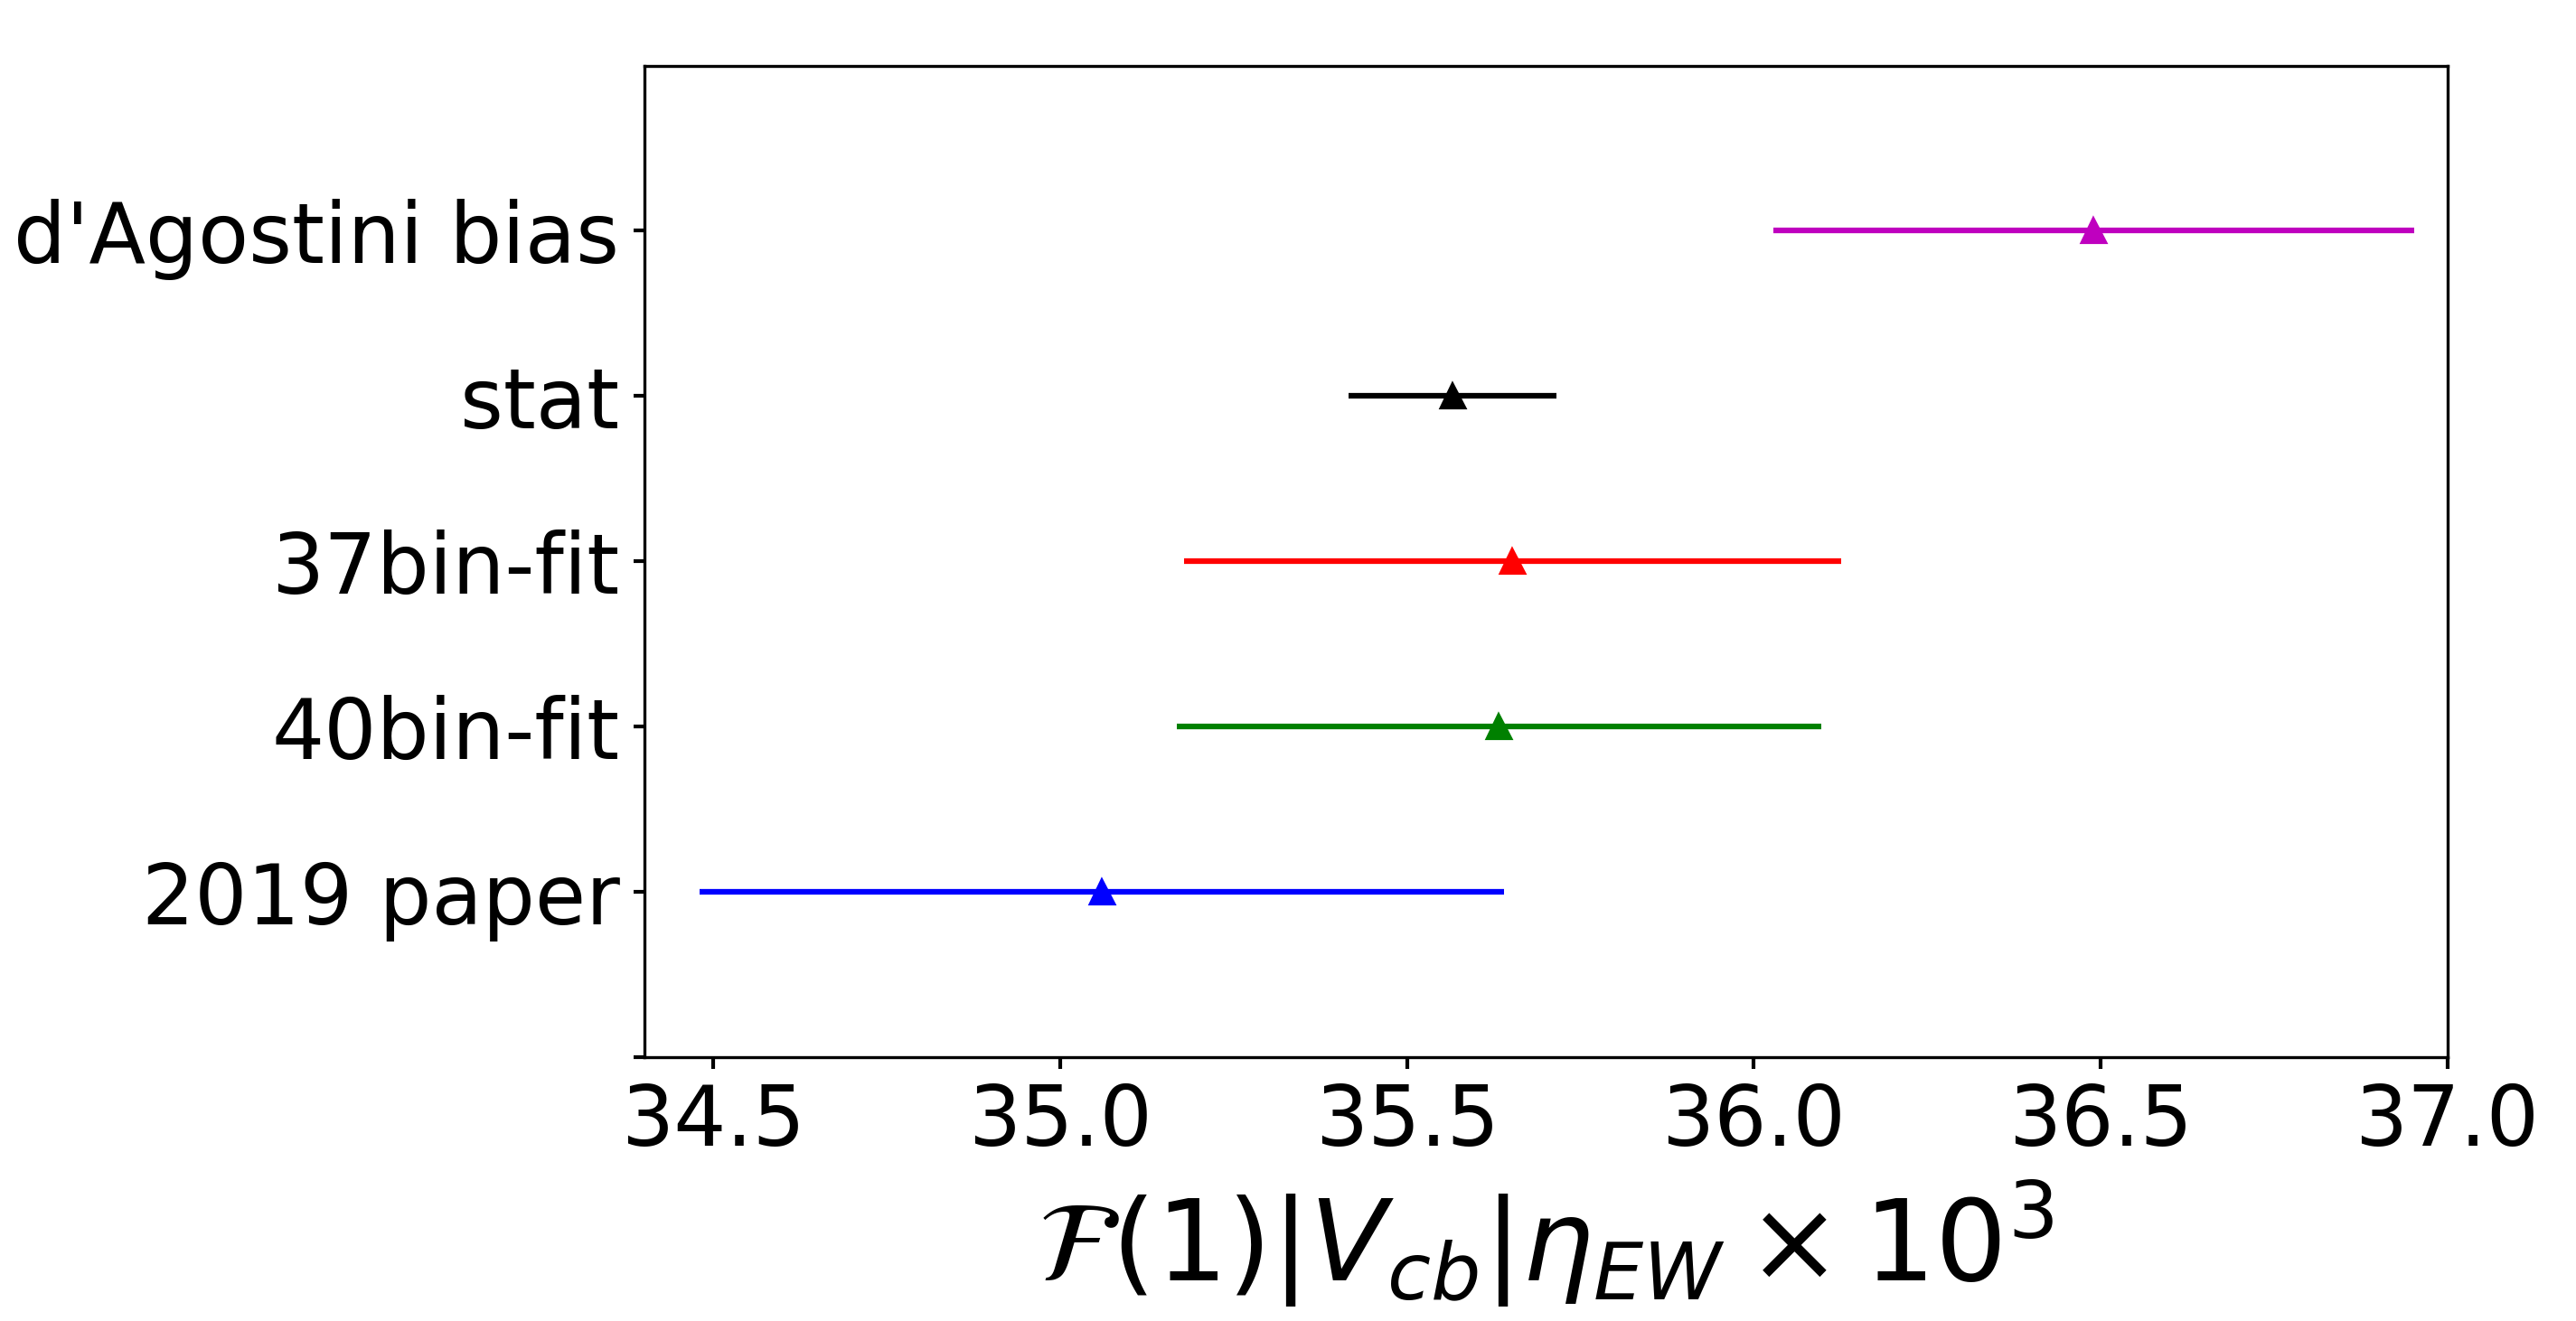
\includegraphics[width=1.0\textwidth]{./Bilder/CLN_all_4}
\end{figure}  
\end{columns}
\vfill
\end{frame}

%%%%%%%%%%%%%%%%%%%%%%%%%%%%%%%%%%%%%%%%%
\begin{frame}{}

  \centering\Huge
  Danke für Ihre Aufmerksamkeit!
\end{frame}

\appendix
%%%%%%%%%%%%%%%%%%%%%%%%%%%%%%%%%%%%%%%%%


%%%%%%%%%%%%%%%%%%%%%%%%%%%%%%%%%%%%%%%%%%%%%%%%%%%%%%%
\begin{frame}{Formfaktor-Parametrisierung}
\footnotesize
\begin{align}
\begin{split}
\frac{d \Gamma   (B^0\longrightarrow D^{*-} \ell ^+ \nu_{\ell})}{dw d \cos \theta_l d \cos \theta_{\nu}d \chi}= & \frac{\eta _{\text{EW}}^2 3 m_{B} m_{D^{*}}^2  }{4 (4 \pi) ^4} G_F^2 |V_{\text{cb}} {}|^2  \sqrt{w^2-1} (1-2wr + r^2)\\
& *\{(1-\cos \theta_l)^2 \sin ^2 \theta_{\nu} H_+^2(w)\\
& +(1+\cos \theta_l)^2 \sin^2\theta_{\nu} H_-^2(w) + 4 \sin^2 \theta_l \cos^2 \theta_{\nu} H_0^2 (w)\\ 
& - 2 \sin^2 \theta_l \sin^2 \theta_{\nu} \cos 2 \chi H_+(w)H_-(w) \\
& - 4 \sin \theta_l (1-\cos \theta_l) \sin \theta_{\nu} \cos \theta_{\nu} \cos \chi H_+(w)H_0(w) \\
& + 4 \sin \theta_l (1+\cos \theta_l) \sin \theta_{\nu} \cos \theta_{\nu} \cos \chi H_-(w)H_0(w)\}
\end{split}
\end{align}
\begin{align}
H_i(w)=m_{B} \frac{R^* \left(1-r^2\right)  (w+1) }{2 \sqrt{1-2 w r +r^2}} h_{\text{A1}}(w) |\tilde{H_i}(w)|
\end{align}

\begin{align}
\tilde{H_\pm}(w)=\frac{\sqrt{1-2 w r +r^2} \left( 1 \mp \sqrt{\frac{w-1}{w+1}} R_1(w) \right)}{(1-r)} 
\end{align}

\begin{align}
\tilde{H_0}(w)=1+ \frac{(w-1)(1-R_2(w))}{(1-r)}
\end{align}
\end{frame}


%%%%%%%%%%%%%%%%%%%%%%%%%%%%%%%%%%%%%%%%%%%%%%%%%%%%%%%
\begin{frame}{Ergebnisse}
\begin{columns}
\column{.5\textwidth}
\begin{figure}[htbp]
   \centering
    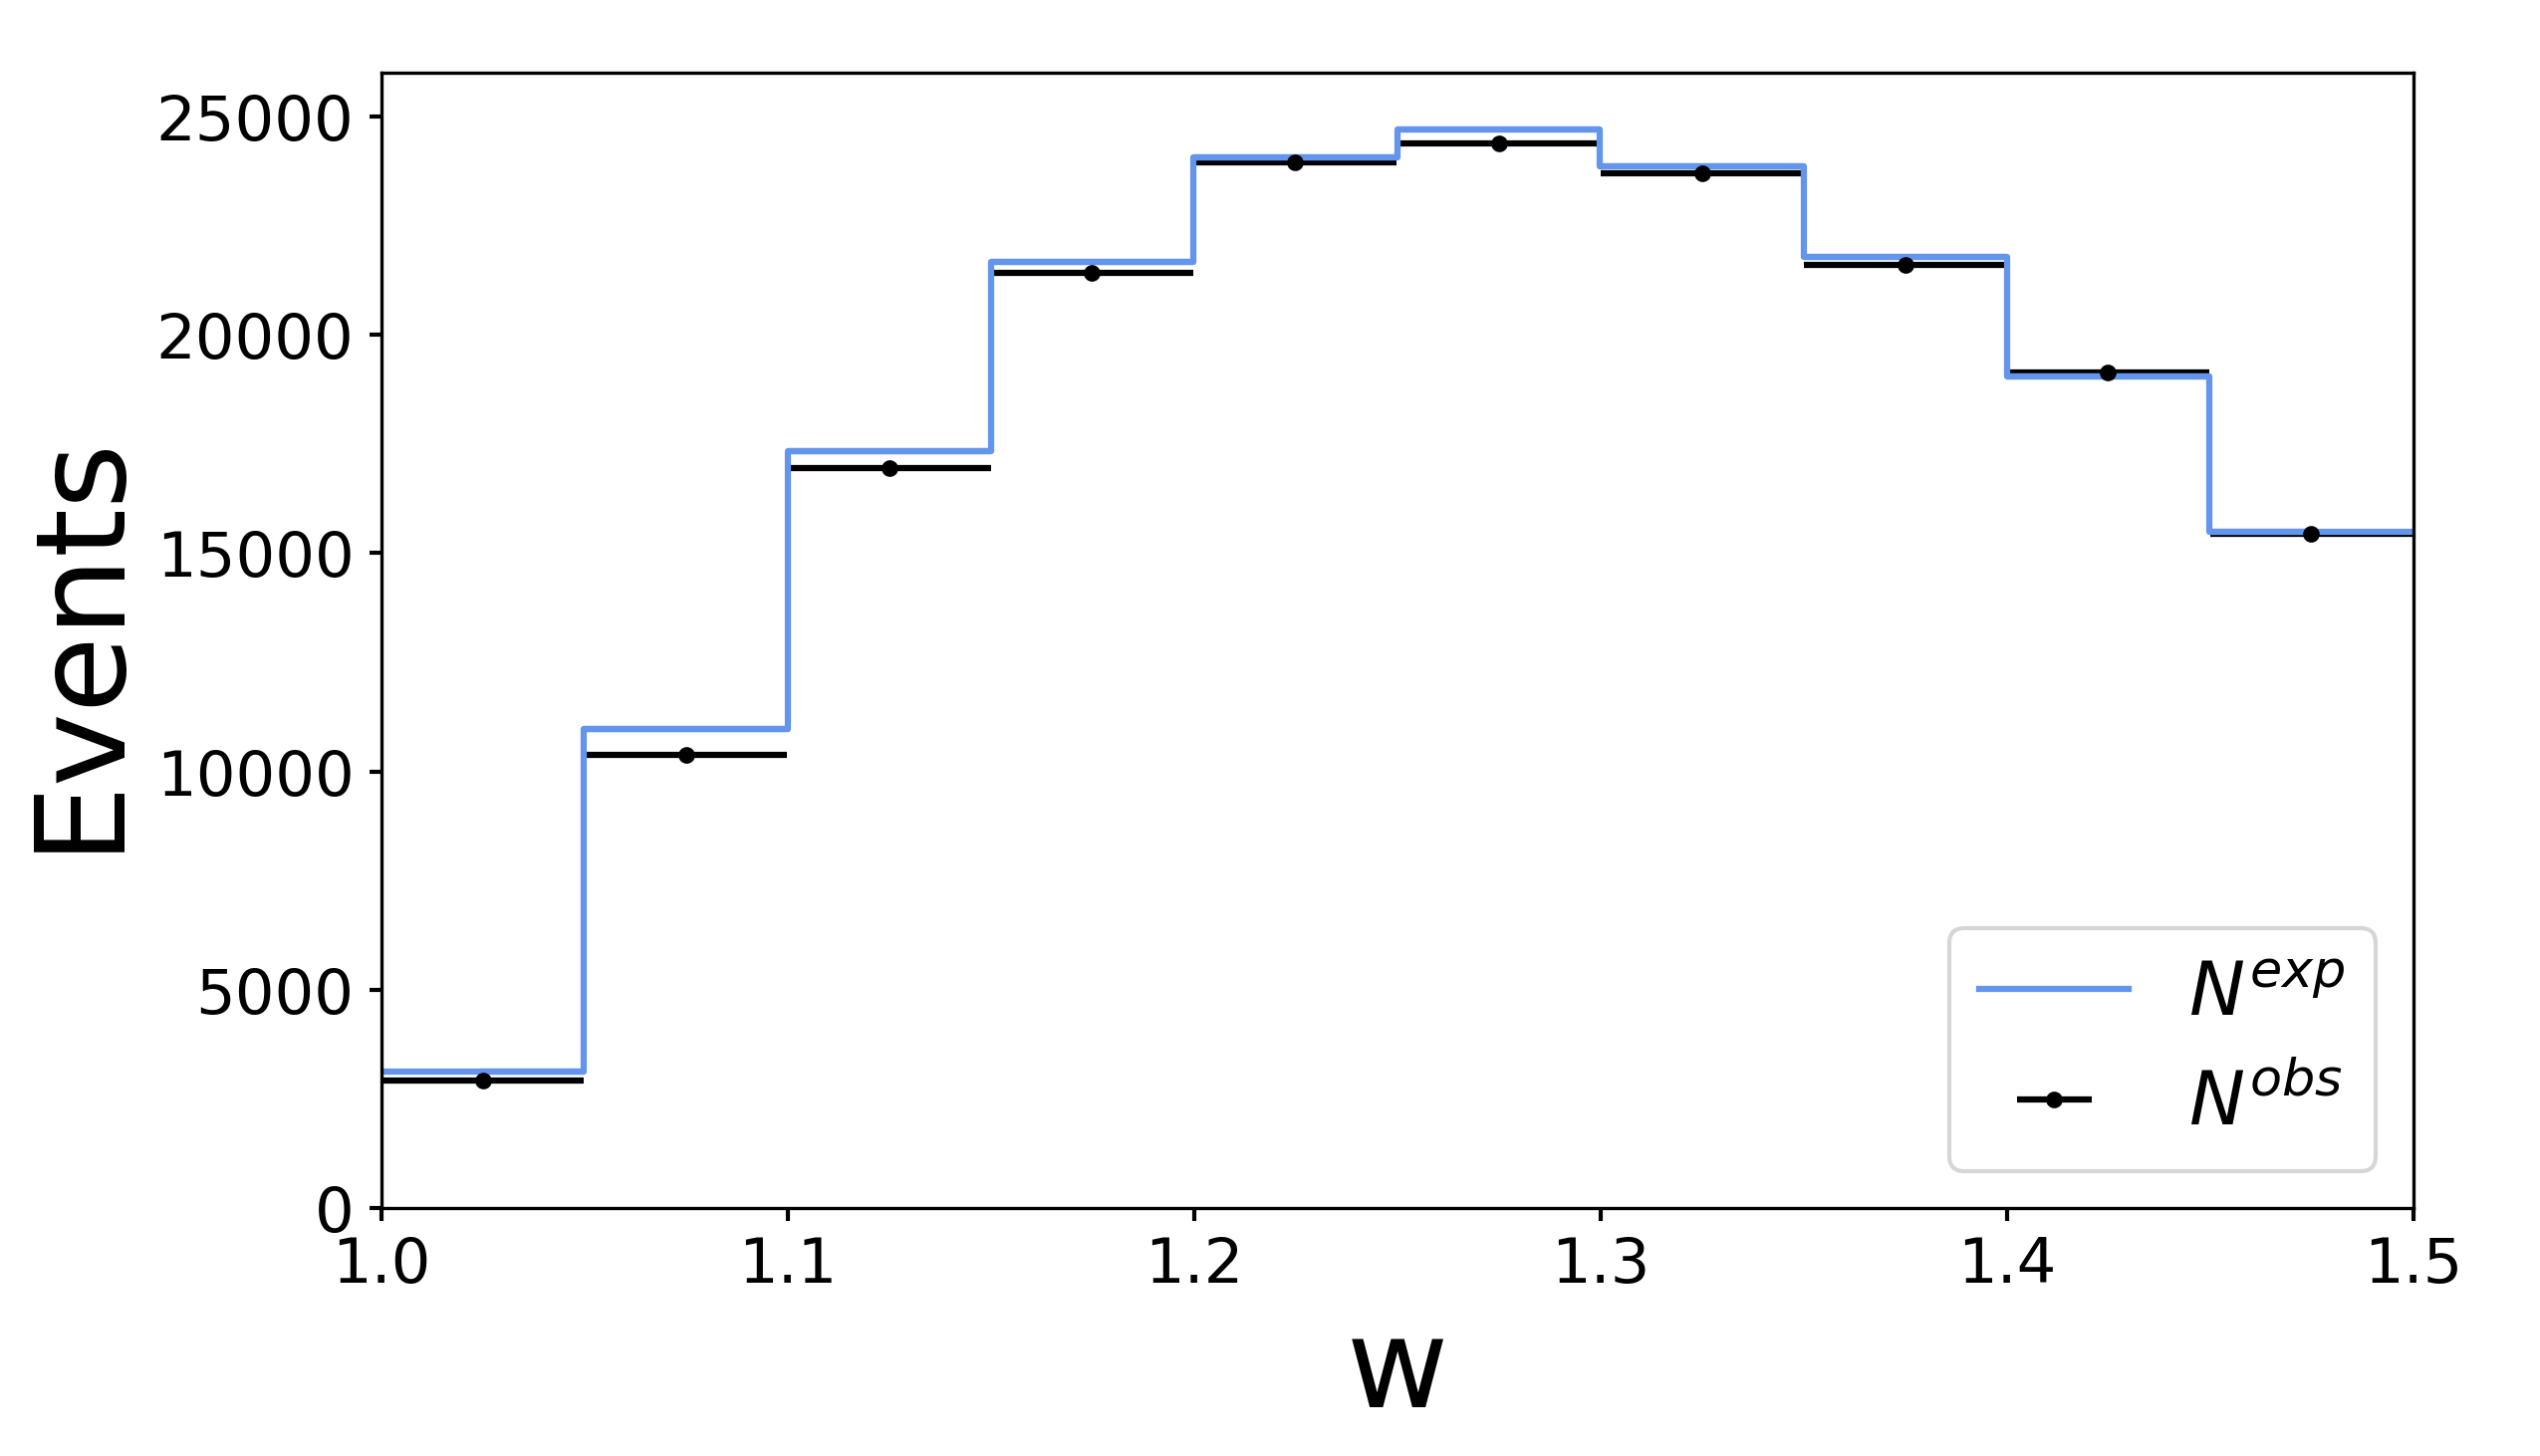
\includegraphics[width=0.7\textwidth]{./Bilder/CLN_em1}
    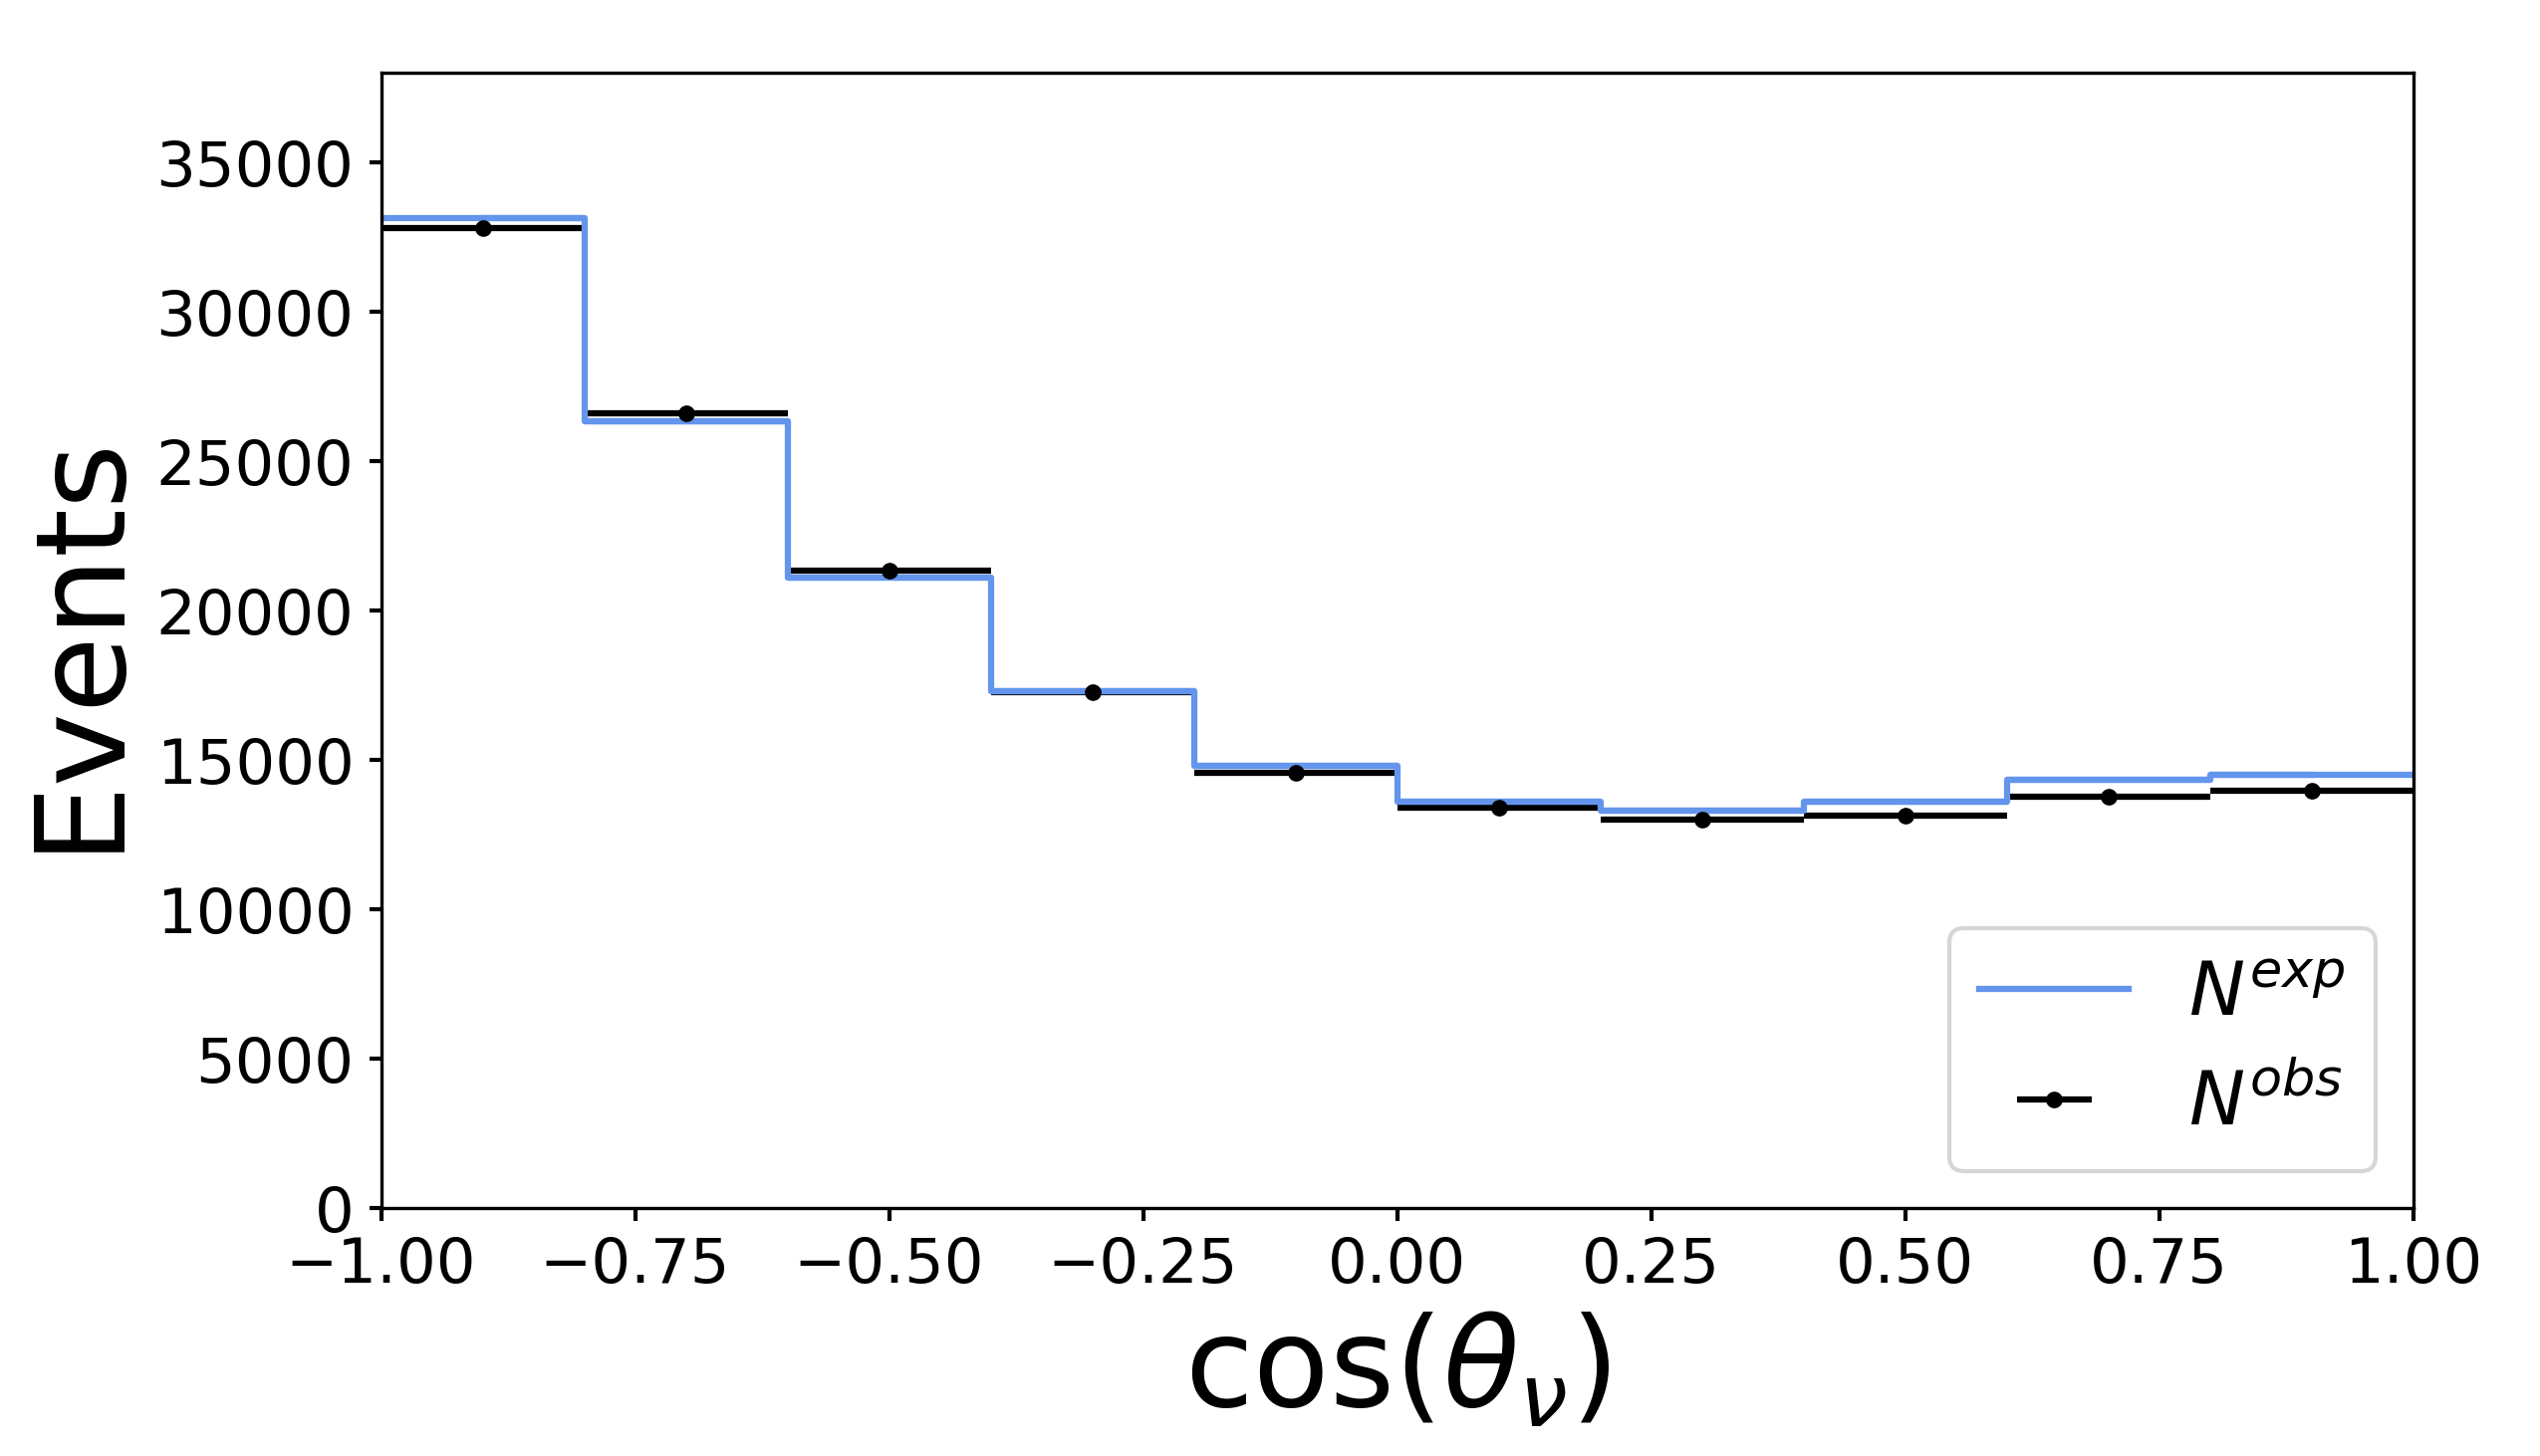
\includegraphics[width=0.7\textwidth]{./Bilder/CLN_em3}
\end{figure}  
\column{.5\textwidth}
\begin{figure}[htbp]
   \centering
    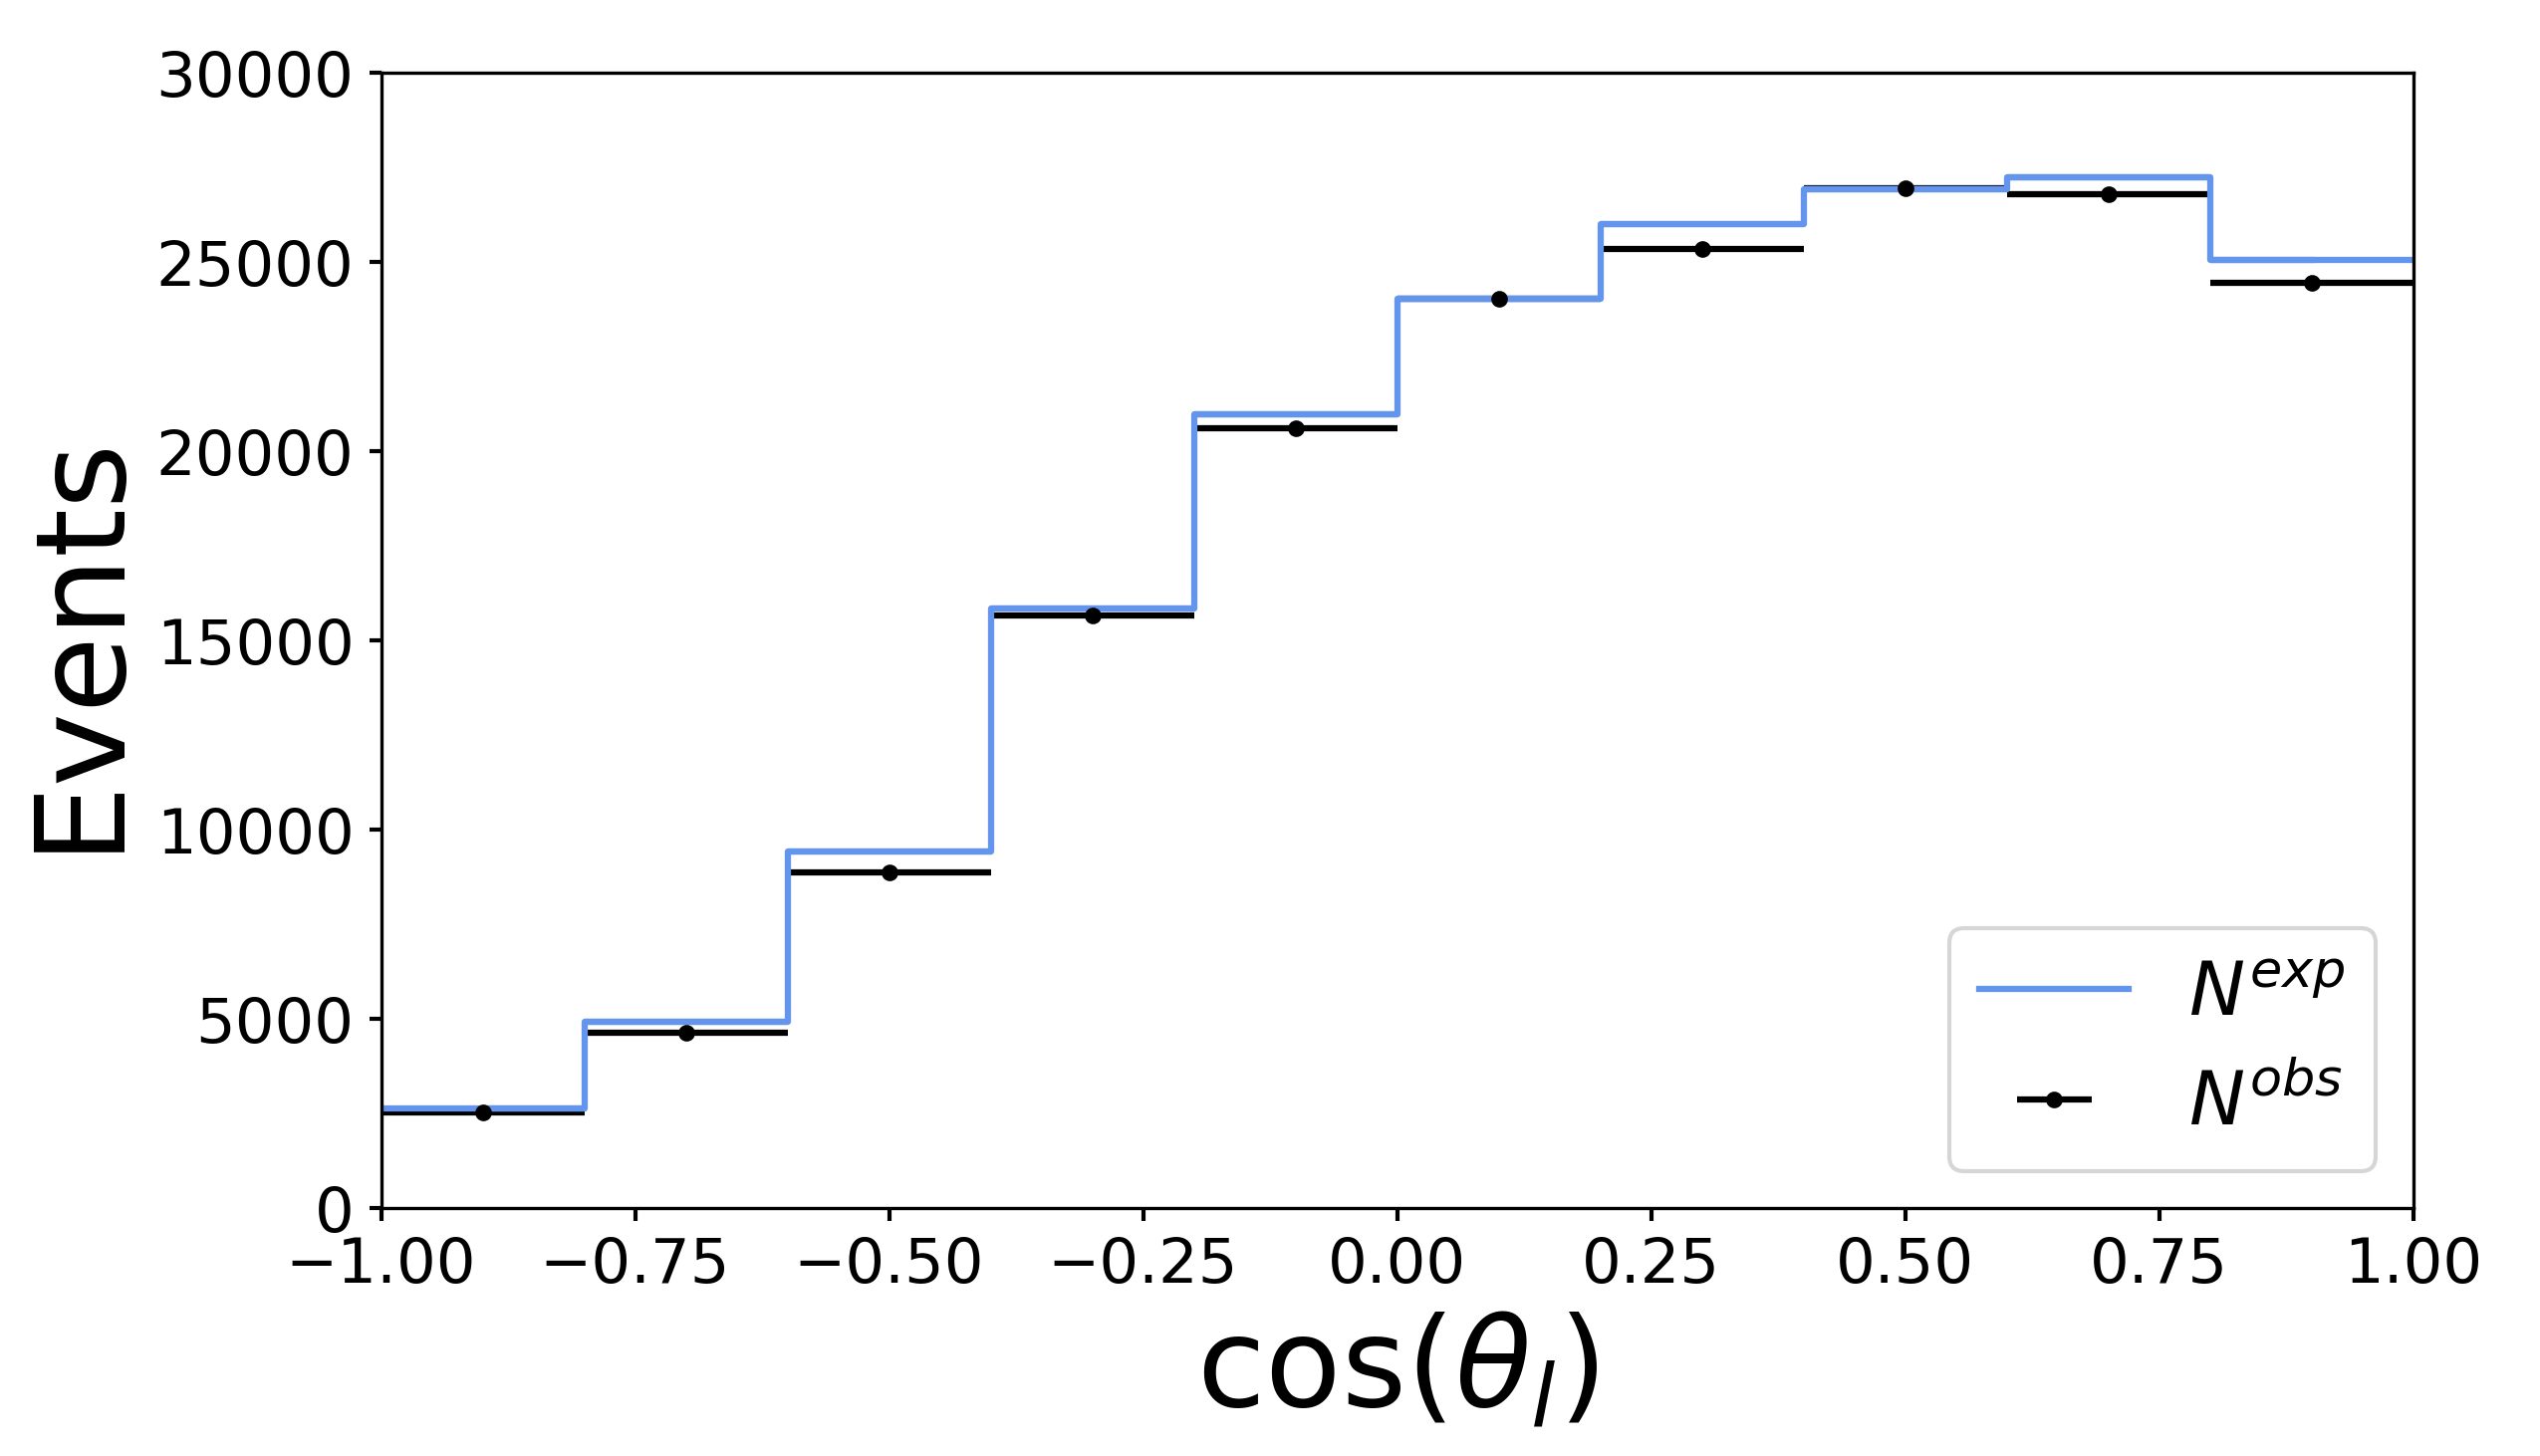
\includegraphics[width=0.7\textwidth]{./Bilder/CLN_em2}
    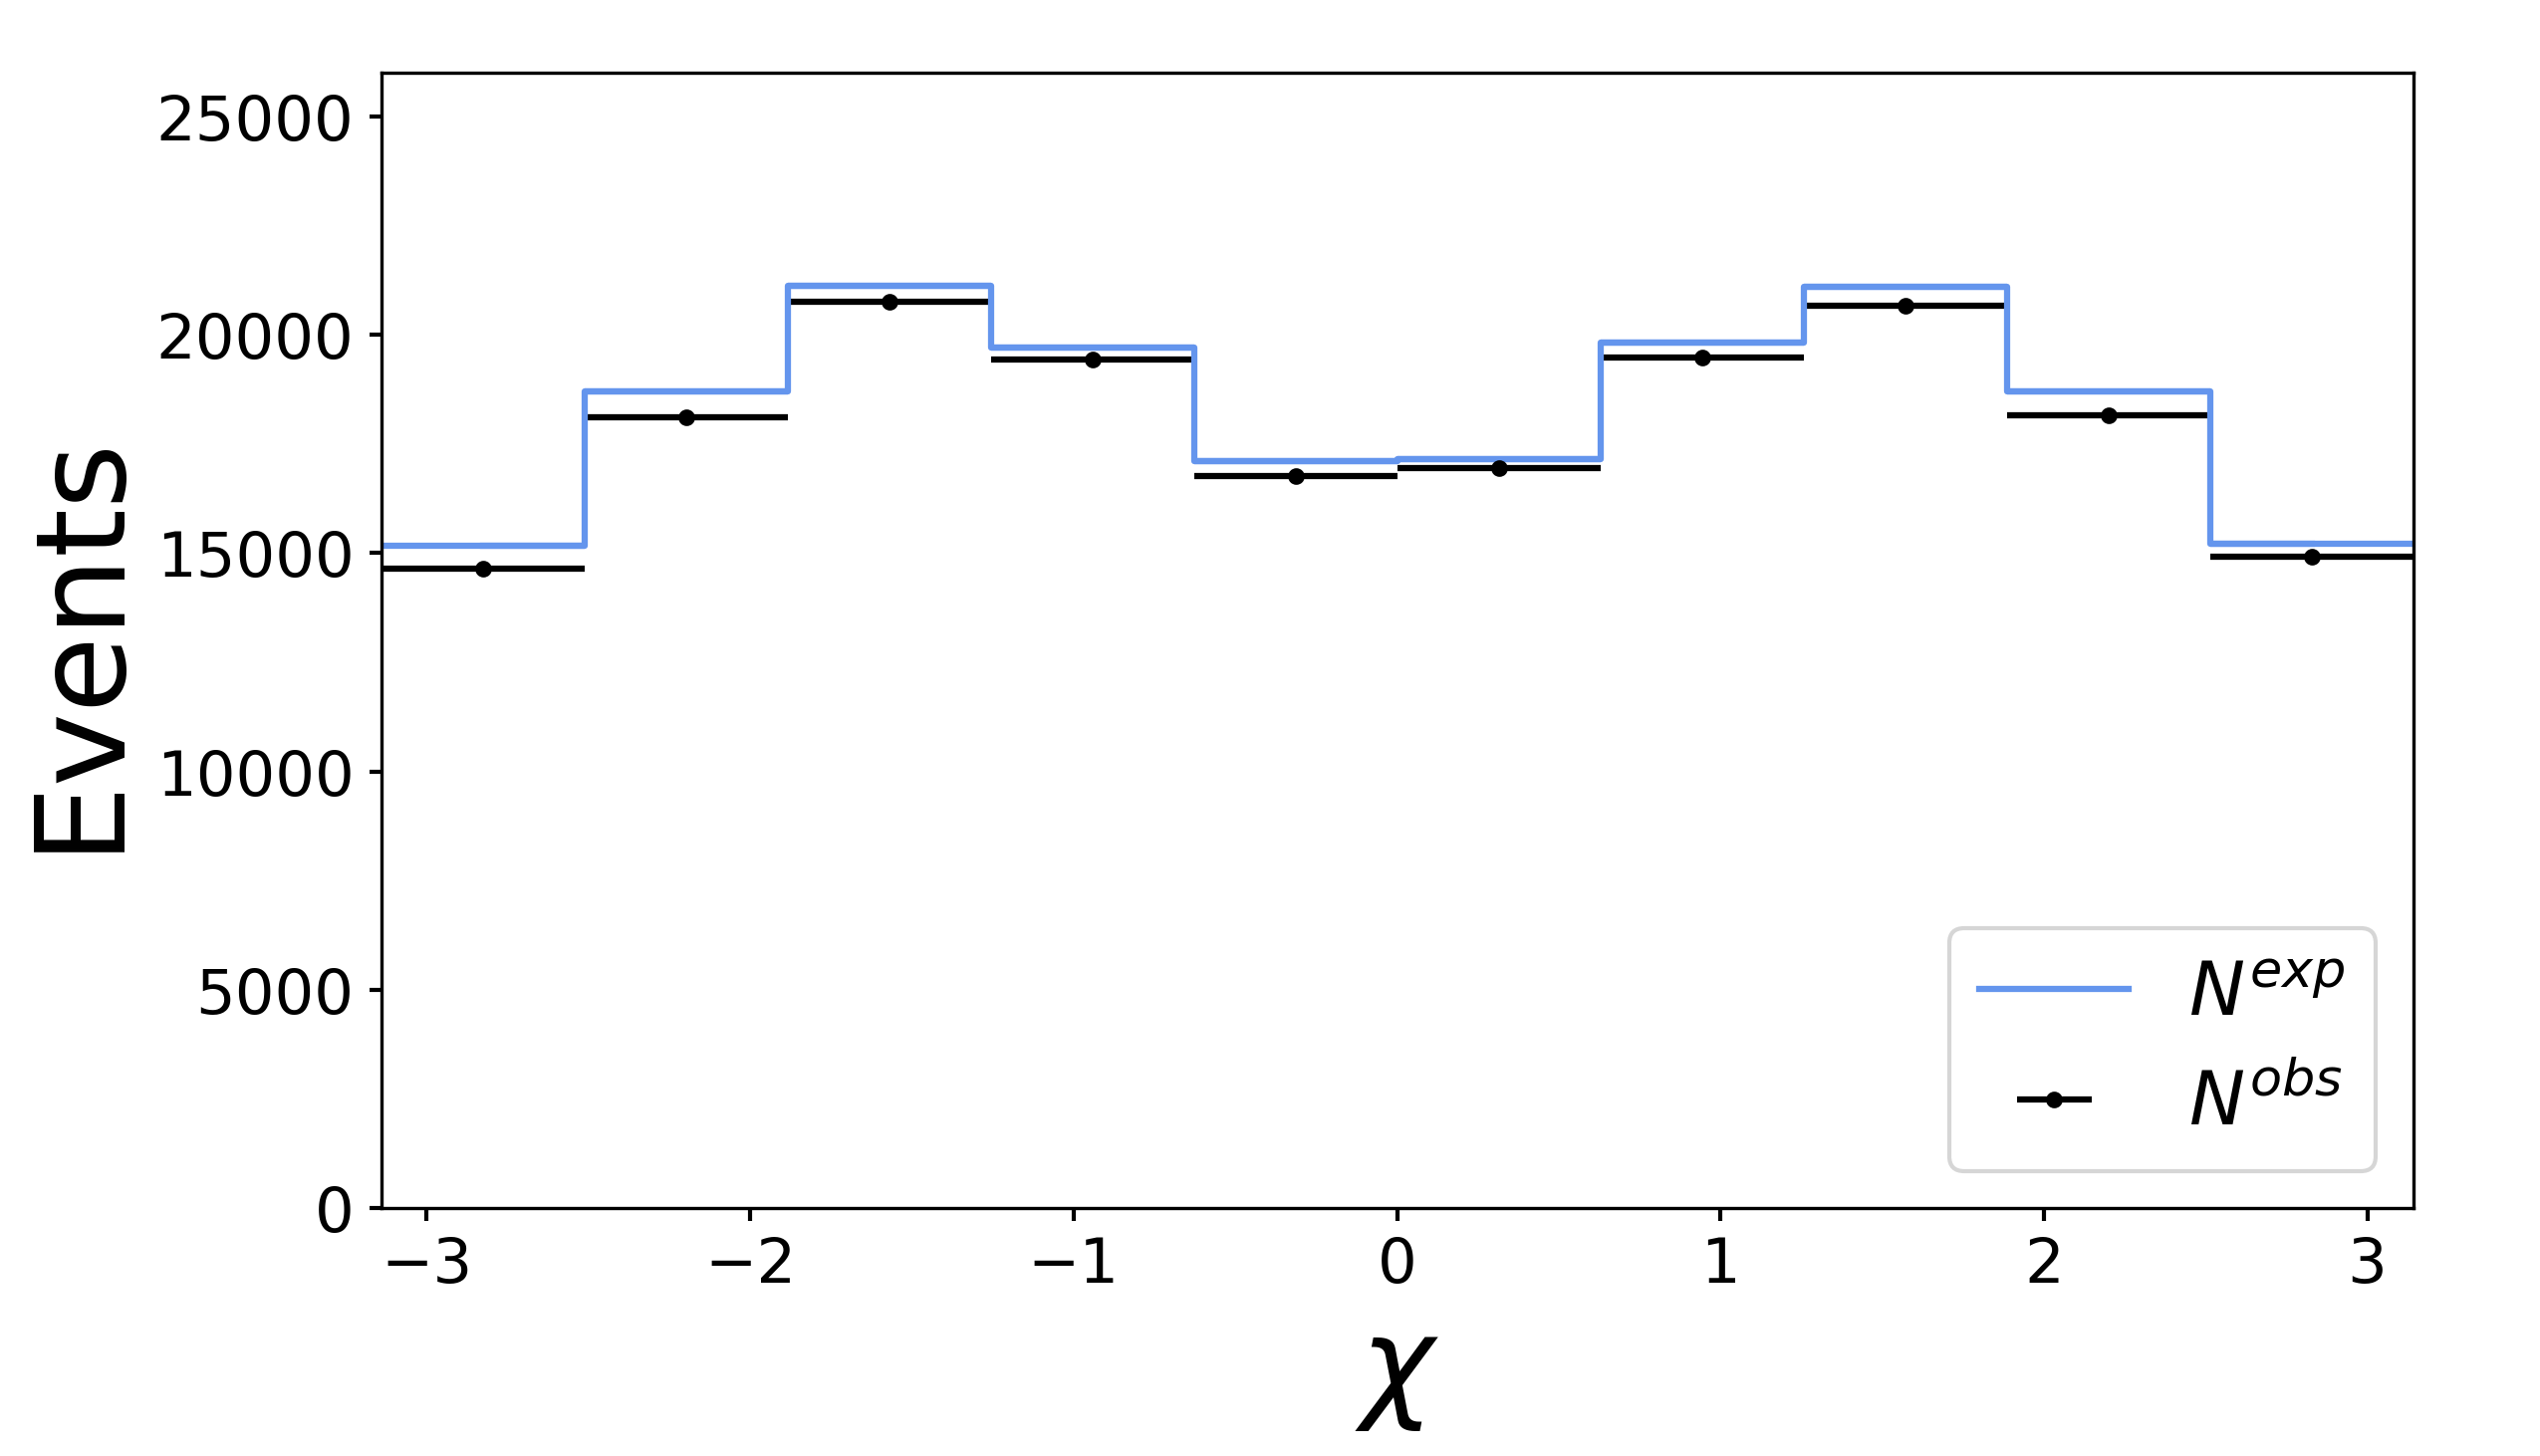
\includegraphics[width=0.7\textwidth]{./Bilder/CLN_em4}
\end{figure}  
\end{columns}
\centering
\small
\begin{tabular}{rl}
$\rho ^2$ = &	$1.166 \pm 0.034 $	\\
$R_1(1)$	 = & $1.184 \pm 0.028 $	 \\
$R_2(1)$		= &	$0.848 \pm 0.022$	 \\
$\mathcal{F} (1) |V_{cb}| \eta _{\text{EW}} \times 10^3$		= &	$36.49 \pm 0.46$	\\ 
\end{tabular} 

\end{frame}


\end{document}

% Lists frame
\section{Lists in Beamer}
\begin{frame}{Lists in Beamer}

This is an unordered list:
\begin{itemize}
    \item Item 1
    \item Item 2
    \item Item 3
\end{itemize}

and this is an ordered list:
\begin{enumerate}
    \item Item 1
    \item Item 2
    \item Item 3
\end{enumerate}

\end{frame}


% Blocks frame
\section{Blocks in Beamer}
\begin{frame}{Blocks in Beamer}
    \begin{block}{Standard Block}
        This is a standard block.
    \end{block}
    \begin{alertblock}{Alert Message}
        This block presents alert message.
    \end{alertblock}
    \begin{exampleblock}{An example of typesetting tool}
        Example: MS Word, \LaTeX{}
    \end{exampleblock}
\end{frame} 

